%------------------------------------------------------------------------------
% This is a LaTeX template for the scientific justification of IRAM Proposals 
%------------------------------------------------------------------------------
% 
% We encourage IRAM proposers to use this template for the sake of unity 
% and clarity when Program Committee members assess their proposals.
% 
% You may customize this template to suit your preferences (e.g. using BibTex),
% but please respect the following requirements:
%     The scientific justification should contain a maximum of 2 pages of text 
%     (4 pages for Large Programs), plus 2 pages of Figs., Tables and Refs.
%     The font size should be 11pt or larger.
%
% For Large Programs, the following sections should be included: 
%   i) Scientific Rationale, 
%  ii) Immediate Objective, 
% iii) Feasibility and Technical Justification, and 
%  iv) Organizational Issues.
% 
%
%------------------------------------------------------------------------------
%
\documentclass[10pt,a4paper,twoside,graphicx,color]{article}
%
\usepackage[margin=2cm]{geometry}
\usepackage[pdftex]{graphicx}
\usepackage{color}
\usepackage{txfonts}
\usepackage{paralist}
\usepackage[numbers]{natbib}
\setlength{\bibsep}{0.0pt}
\usepackage{amssymb}
\usepackage{hyperref}
\newcommand{\ccor}[1]{\textcolor{red}{#1}}

\bibpunct{(}{)}{;}{a}{}{,} % to follow the A&A style
\bibliographystyle{aa} % style aa.bst

%
% Page size and text dimensions
% Do not change!
\textheight 260mm
\textwidth 178mm
\oddsidemargin -8mm
\evensidemargin -8mm
\marginparwidth 50pt
\topmargin -22mm
\brokenpenalty=10000
\sloppy
%
%-------------------------------------------------------------------
\begin{document}
%
%
\begin{center}{\huge \bf
%-------------------------------------------------------------------
ARSENAL: intermediAte Redshift Sz clustEr NikA2 time fiLler: a demo run
%-------------------------------------------------------------------
}\end{center}
% 
\begin{center}
F.X. D\'esert (IPAG), the NIKA2 core team, et al.
\end{center}

%-------------------------------------------------------------------
\vspace{-0.3cm}
%\section{Scientific context}
%\vspace{-0.3cm}
       {\bf Abstract -- } Clusters of galaxies are invaluable tools
       for measuring cosmological parameters. The SZ effect directly
       measures the baryon pressure inside clusters. We suggest to
       optimize the use of the 30m with a Time Filler proposal that
       will span several years. Here we only request time (20~hours)
       to demonstrate the usefulness of such a survey. The survey is a
       direct follow-up of the {\sl Planck} clusters. It consists in
       mapping the SZ effect at 2~mm, on a selected sample of
       intermediate redshift clusters (typically 0.15 to 0.3) for
       which many complementary data are available. The published end
       products would be calibrated maps of the $y$ Compton parameter
       and a point-source catalog per cluster. Derived parameters
       include the cluster pressure profile, the presence of shocks,
       substructures, and possibly, the total mass and the baryonic
       mass.\\

       %Combined with {\sl Planck} data, we can measure the Hubble Constant and the baryon-to-total mass ratio.



\vspace{-0.1cm} \noindent {\bf \large Scientific context -- } Clusters
of galaxies are the most massive collapsed structures in the
Universe. They have been used as a probe of the matter content on
large scales. As early as in 1933, \cite{Zwicky1933} demonstrated that
there was a lot more matter than meets the eye (of optical observers)
in clusters of galaxies. Since then, it has been established that dark
matter dominates the mass budget of clusters of galaxies, the hot gas
being the major baryonic component and the galaxies being a minor
constituent. The hot gas has been thoroughly observed with X-ray
telescopes, the later ones being XMM and Chandra. The interaction of
the Cosmic Microwave Background with the hot electrons is called the
Sunyaev-Zel'dovich (SZ) effect (\cite{SZ1972}). It produces a
brightness decrement at the cluster location at the NIKA2 wavelength
of 2~mm.  The {\sl Planck} satellite (\cite{PSZ2}), ACT
(\cite{Hasselfield2013}) and SPT (\cite{Bleem2014}) have produced the
biggest catalogs of SZ observations, with thousands of clusters being
measured. The millimetre observations are complementary to X-rays. The
X-ray emissivity is mostly proportional to the square of the density,
whereas the SZ effect is directly sensitive to the pressure along the
line-of-sight and globally, to the total thermal energy of the
cluster. In combination, the two measurements allow disentangling the
density and temperature parameters. At intermediate redshifts (0.15 to
0.3), the clusters have been well observed by X-ray satellites. But
the SZ picture offers a less biased view of the baryonic content of a
cluster. 
%Large SZ cluster surveys, such as those by the ACT (e.g., Hincks et al. 2010 and Marriage et al. 2011), SPT (e.g. Vanderlinde et al. 2010, Carlstrom et al. 2011, Williamson et al. 2011 and Reichardt et al. 2013) and {\sl Planck} (e.g. Tauber et al. 2010 and {\sl Planck} Collaboration et al. 2011) 
Fig.~\ref{Fig:AllSky} shows all the clusters of galaxies detected by
{\sl Planck}: they are everywhere on the sky and therefore constitute
perfect targets for a time-filler ground-based follow-up survey which
is considered here. The large majority of {\sl Planck} clusters are in
the redshift range we are targetting. For many clusters, the
millimetre data are scarce and the complementarity of that survey with
data from reference 2000-2030 missions like {\sl Herschel, XMM,
  Chandra, Euclid, eRosita, LOFAR, SKA, Athena} is
clear. Fig.~\ref{Fig:SZprofile} (right) shows the lack of SZ maps in
the center of clusters of intermediate redshift. The core radius of
intermediate redshift clusters is about 1-2 arcminutes (corresponding
to few hundreds kilopc). The 2~mm signal follows a
$(1+\frac{\theta^2}{\theta_c^2 })^{-0.8}$ law, where $\theta$ is the
angular radius to the center and $\theta_c$ is the angular core
radius. This is represented in Fig.~\ref{Fig:SZprofile}. Mapping the
center of clusters would reveal their dynamical state and, in
particular, if they are perturbed or not, and if they posess a
cool-core (the cooling time is shorter than the Hubble time) or not
(see {\sl e.g.} \cite{Hudson2010}). \\


\vspace{-0.1cm} \noindent {\bf \large Main scientific goals -- } The
proposed SZ mapping of clusters of galaxies will directly provide: 1--
high angular resolution (18~arcsecond) $y$ Compton parameter maps of
well-known clusters. So far, the SZ maps were obtained with a low to
mid resolution beams. For example, the {\sl Planck} beam at 2~mm is
7~arcminute, barely resolving even the biggest clusters. ACT and SPT
have also provided catalogs of clusters of galaxies which also suffer
from mid angular resolution. An impressive catalog of SZ maps has been
obtained by Carlstrom et al.~(right side of Fig.~\ref{Fig:AllSky}) at
15~GHz (OVRO/BIMA, 1.7 to 2.8~arcmin resolution, \cite{Reese2002}). We
want to extend that pionneer survey in terms of the number of
clusters, the frequency and the angular resolution. The proposed maps
would cover only the central part of the clusters. The external part
has already been mapped with unprecedented accuracy by {\sl
  Planck}. 2-- A catalog of 2~mm sources. They will be mostly radio
sources (e.g. the Brightest Cluster Galaxy). The submillimetre
galaxies cannot be detected with the poor sensitivity expected at
1~mm. Herschel catalogs will be used in any case to take into account
potential contaminations. 3-- Central pressure profiles of a large
sample of clusters. From these profiles and X-ray data from
XMM-Newton, one can infer the baryonic mass (dominated by the hot
plasma outside the galaxies) and the total mass of the cluster, via
the hydrostatic hypothesis, in combination with X-ray and {\sl Planck}
data. 4-- Inhomogeneities can reveal AGN feedback, shocks, X-ray bubbles and
substructures which can be correlated with X-rays and low-frequency
radio surveys (relics, and so on) as LOFAR, and, in the future,
SKA. This is revealing the dynamics and agregation of clusters within
their supercluster environment. The main goal of this proposal is to
make a {\sl Planck} ground-based followup, with maps at high angular
resolution of a large sample of the center of individual clusters. The
{\sl Planck} measurement suffers from the very imperfect knowledge of
the cluster size and central details
(\cite{Planck2013PressProf}). This could potentially improve the
accuracy of the {\sl Planck} cosmological constraints coming from
clusters of galaxies.
%If possible, we can also measure the Hubble constant without the use of the canonical cosmic ladder and study the substructures within clusters of galaxies. For example, Reese etal (2002) used 18 clusters, observed with OVRO/BIMA, to determine the Hubble constant as $60\pm4\mathrm{km s^{-1}Mpc^{-1}}$, with a systematic error error bar 4 times larger.\\
Other outputs of this survey include serendipitous ones: odd sources,
map features. A sure output will be a complementary dataset on
clusters, which are studied at many other wavelengths (including
deeper maps with NIKA2 at 1 and 2~mm). In that respect, we intend to
publish the survey results in an open database. Cluster maps would be
public within a year of observations. In relation to the ongoing
Guaranteed Time NIKA2 SZ Large Program on clusters of galaxies, we
think that it is very complementary because: here we aim at
intermediate redshift clusters (0.15 to 0.3) which are more extended
and in shallow mode observations, whereas the LPSZ survey aims at high
redshift ($z\ge 0.5$) clusters observed with high sensitivity down to
their edges, and with a thorough control of sources that can perturb
the maps (hence the importance of the 1~mm channel). Other instruments
have already followed-up on {\sl Planck} clusters in order to make SZ
maps at better resolutions: AMI (a UK 15~GHz interferometer) in
particular has been used and provided observations of 123~clusters,
including 99~detections (\cite{Perrott2015}), each observation
requiring 60~hours of integration with a limited angular resolution of
3~arcminutes.\\

\vspace{-0.1cm} \noindent {\bf \large Feasability and Sample selection
  -- } Observing intermediate redshift clusters requires to map
angular scales of the order of the NIKA2 field-of-view. The findings
within the NIKA2 collaboration is that scales mapped within less than
3~seconds can be recovered while larger scales suffer from various
low-frequency noises (sky noise and electronic noise mostly) that are
difficult to remove with decorrelation techniques. Scanning fast
``freezes'' the atmosphere. With a FOV diameter of 390~arcseconds, it
becomes important to map at a speed larger than about
100~arcsecond/s. With 150, the sampling of NIKA2 (at the standard
23~Hz acquisition) is 6.5~arcseconds which is not really compatible
with Nyquist sampling of the 12~arcseconds 1~mm beam. Whenever
necessary, we should therefore go to the fast acquisition rate (46~Hz)
which is used in the polarimetric mode, without enabling the half-wave
plate here. Operationnally, the switching time is of a few minutes. A
speed of 160 arcseconds/s is within the 30~m capabilities without loss
of pointing accuracy. We show in Fig.~\ref{Fig:1sqdegMap} an example
of such a scanning speed capability. In this proposal, we request
observing the targets given in the Table in order to have a
demonstration opportunity. We want to show that that survey can be
done with the requirements that we need: 1) the scan speed can
increase the recovery of large angular scales and the images are
reproducible, even though the opacity is mediocre, 2) the pointing
does not need to be accurate at all (4~arcseconds) 3) the sky noise
has been discussed above, 4) the survey is insensitive to the 1~mm
conditions, 5) the beam must not be perfect but reproducible, 6)
anomalous refraction should be limited. 7) opacity correction does not
limit the calibration accuracy.\\

We need to achieve a $y$ sensitivity below $10^{-4}$ for one beam so
that the center of the cluster (typically with a central $y$ of
$3\times 10^{-4}$) can be well mapped. The size of the clusters being
below 8~arcminutes, scans of 20 by 12 arcminutes at 4 different
orientations (0, 45, 90, 135~degrees) in Ra-Dec coordinates are
required to obtain a central 12~arcminute diameter map and enough
blank fields around to set the zero level. With a maximal azimuth
speed of the telescope of 170~arcsecond/s, an effective scanning speed
of 120 (resp. 83) arcsec/s can be achieved at an elevation of 45
(resp. 60) degrees. The trade-off between speed and opacity (due to
the low elevation) will have to be made on a cluster-to-cluster
basis. The integration time can be roughly estimated by assuming an
average mediocre zenith opacity of 0.5 at 2~mm (0.75 for the 225~GHz
IRAM taumeter!) and an elevation of 45~degrees so that the sensitivity
becomes $20\,\mathrm{mJy.s^{1/2}}$ per detector. The conversion from
Jy to $y$ involves a factor 12 so that the $y$ $1\,\sigma$ sensitivity
for 1~hour is $20\times 10^{-3}/12/\sqrt{3600\times 0.7}=2.3\times
10^{-5}$ for one field-of-view and adopting 0.7 for the number of
valid Kids. The scan involves an area of $20\times
12\,\mathrm{arcmin^2}$ which covers 7~FOV, so the final sensitivity of
the central 12~arcmin map, after 2~hours (total integration time),
will be, in $y$ terms, of $2.3\times 10^{-5}\sqrt{7/2}=4.3\times
10^{-5}$. Even after accounting for diffuse vs. point-source
sensitivities, this is well below the target sensitivity of
$10^{-4}$. It would provide a Signal-to-Noise ratio at the peak of 10
per beam (depending on the central strength of the cluster), while the
signal covers several square-arcminutes. Fig.~\ref{Fig:SZprofile}
shows a typical profile and error bars in annuli that are expected for
massive clusters. Including an overhead of 2 for calibration and
pointing, the demonstration of the time-filler proposal could be done
with the observation of 5~clusters, each of them with a duration of
4~hours. We therefore request {\bf 20~hours} of observations with
NIKA2, using only the weather conditions where standard NIKA2
proposals cannot be scheduled. This project could be a pathfinder
projects for other large-scale 2~mm mapping projects. The team has a
lot of experience in the data reduction of SZ observations of clusters
of galaxies with NIKA and NIKA2, and reuse of available IDL sofware is
planned (\href{https://ipag.osug.fr/nika2/Publications.html}{NIKA2 consortium publications}).
%According to the published commissioning results of the NIKA2 instrument, the total observing time using the NIKA2 2 mm band to map a region of 240.0 [arcmin^2] to reach an rms of 0.5 [mJy/beam], assuming 9.0 [mm] pwv, 45.0 [deg] elevation, Filter = 1.0, Overhead = 2.0, was estimated to be *2.4 hours*, using the time estimator v 2020.JUL.22.


The table of clusters for the whole survey is made of 400 entries
(Fig.~\ref{Fig:RelTau} right). Of course, any source which is being
scheduled for other open time proposals would be withdrawn from this
proposal, but we do not expect to see many cases of fencing.
Fig.~\ref{Fig:RelTau} (left) illustrates that the opacity is between
0.4 and 0.7 for 25~\% of the 30~m time (0.25, 0.5 at 2~mm). Accounting
for typically 3 months of NIKA2, the expected total integration time
for this survey could be of 500 hours per year, allowing to map
hundreds of clusters in several years (with a rolling proposal). The
demo time-filler proposal is here intended to show the capability of
recovering the diffuse emission of clusters of galaxies. It will allow
to ascertain the feasability of the complete time-filler proposal that
we will then submit, if the results are satisfactory. It stems from
our (slight) frustration, as regular NIKA2 observers, of not using
NIKA2 for some lenghty duration because of the opacity
constraints. This survey does not ``cost'' much and would optimize the
use of the NIKA2 instrument with a direct public legacy.\\
% Bibliography and bibfile
\def\aj{AJ}%
          % Astronomical Journal
\def\actaa{Acta Astron.}%
          % Acta Astronomica
\def\araa{ARA\&A}%
          % Annual Review of Astron and Astrophys
\def\apj{ApJ}%
          % Astrophysical Journal
\def\apjl{ApJ}%
          % Astrophysical Journal, Letters
\def\apjs{ApJS}%
          % Astrophysical Journal, Supplement
\def\ao{Appl.~Opt.}%
          % Applied Optics
\def\apss{Ap\&SS}%
          % Astrophysics and Space Science
\def\aap{A\&A}%
          % Astronomy and Astrophysics
\def\aapr{A\&A~Rev.}%
          % Astronomy and Astrophysics Reviews
\def\aaps{A\&AS}%
          % Astronomy and Astrophysics, Supplement
\def\azh{AZh}%
          % Astronomicheskii Zhurnal
\def\baas{BAAS}%
          % Bulletin of the AAS
\def\bac{Bull. astr. Inst. Czechosl.}%
          % Bulletin of the Astronomical Institutes of Czechoslovakia 
\def\caa{Chinese Astron. Astrophys.}%
          % Chinese Astronomy and Astrophysics
\def\cjaa{Chinese J. Astron. Astrophys.}%
          % Chinese Journal of Astronomy and Astrophysics
\def\icarus{Icarus}%
          % Icarus
\def\jcap{J. Cosmology Astropart. Phys.}%
          % Journal of Cosmology and Astroparticle Physics
\def\jrasc{JRASC}%
          % Journal of the RAS of Canada
\def\mnras{MNRAS}%
          % Monthly Notices of the RAS
\def\memras{MmRAS}%
          % Memoirs of the RAS
\def\na{New A}%
          % New Astronomy
\def\nar{New A Rev.}%
          % New Astronomy Review
\def\pasa{PASA}%
          % Publications of the Astron. Soc. of Australia
\def\pra{Phys.~Rev.~A}%
          % Physical Review A: General Physics
\def\prb{Phys.~Rev.~B}%
          % Physical Review B: Solid State
\def\prc{Phys.~Rev.~C}%
          % Physical Review C
\def\prd{Phys.~Rev.~D}%
          % Physical Review D
\def\pre{Phys.~Rev.~E}%
          % Physical Review E
\def\prl{Phys.~Rev.~Lett.}%
          % Physical Review Letters
\def\pasp{PASP}%
          % Publications of the ASP
\def\pasj{PASJ}%
          % Publications of the ASJ
\def\qjras{QJRAS}%
          % Quarterly Journal of the RAS
\def\rmxaa{Rev. Mexicana Astron. Astrofis.}%
          % Revista Mexicana de Astronomia y Astrofisica
\def\skytel{S\&T}%
          % Sky and Telescope
\def\solphys{Sol.~Phys.}%
          % Solar Physics
\def\sovast{Soviet~Ast.}%
          % Soviet Astronomy
\def\ssr{Space~Sci.~Rev.}%
          % Space Science Reviews
\def\zap{ZAp}%
          % Zeitschrift fuer Astrophysik
\def\nat{Nature}%
          % Nature
\def\iaucirc{IAU~Circ.}%
          % IAU Cirulars
\def\aplett{Astrophys.~Lett.}%
          % Astrophysics Letters
\def\apspr{Astrophys.~Space~Phys.~Res.}%
          % Astrophysics Space Physics Research
\def\bain{Bull.~Astron.~Inst.~Netherlands}%
          % Bulletin Astronomical Institute of the Netherlands
\def\fcp{Fund.~Cosmic~Phys.}%
          % Fundamental Cosmic Physics
\def\gca{Geochim.~Cosmochim.~Acta}%
          % Geochimica Cosmochimica Acta
\def\grl{Geophys.~Res.~Lett.}%
          % Geophysics Research Letters
\def\jcp{J.~Chem.~Phys.}%
          % Journal of Chemical Physics
\def\jgr{J.~Geophys.~Res.}%
          % Journal of Geophysics Research
\def\jqsrt{J.~Quant.~Spec.~Radiat.~Transf.}%
          % Journal of Quantitiative Spectroscopy and Radiative Trasfer
\def\memsai{Mem.~Soc.~Astron.~Italiana}%
          % Mem. Societa Astronomica Italiana
\def\nphysa{Nucl.~Phys.~A}%
          % Nuclear Physics A
\def\physrep{Phys.~Rep.}%
          % Physics Reports
\def\physscr{Phys.~Scr}%
          % Physica Scripta
\def\planss{Planet.~Space~Sci.}%
          % Planetary Space Science
\def\procspie{Proc.~SPIE}%
          % Proceedings of the SPIE
\let\astap=\aap
\let\apjlett=\apjl
\let\apjsupp=\apjs
\let\applopt=\ao
\bibliography{biblio}

Table of  clusters (unfenced according to CDS), among which, 5 will be selected for the Demo proposal\\
name, redshift, coordinates (J2000)\\
A520,  0.202, 04h54m19s,   +02d56.8m,	73.579133, 2.946893 \\
A665,  0.182, 08h30m45s,   +65d52.9m,	127.688306, 65.882026\\
A773,  0.216, 09h17m59s,   +51d42.4m,	139.497459, 51.706411\\
A1413, 0.142, 11h55m18.9s, +23d24m31s,	178.828750, 23.408611\\
A1689, 0.183, 13h11m29.5s, -01d20m17s,	197.872917, -1.338056\\
A1835, 0.252, 14h01m02.3s, +02d52m48s,	210.259583, 2.880000\\
A2163, 0.202, 16h15m34s,   -06d07.4m,   243.892221, -6.123970\\
A2218, 0.176, 16h35m52.4s, +66d12m52s,	248.968333, 66.214444\\

\begin{figure}
  \begin{center}
   %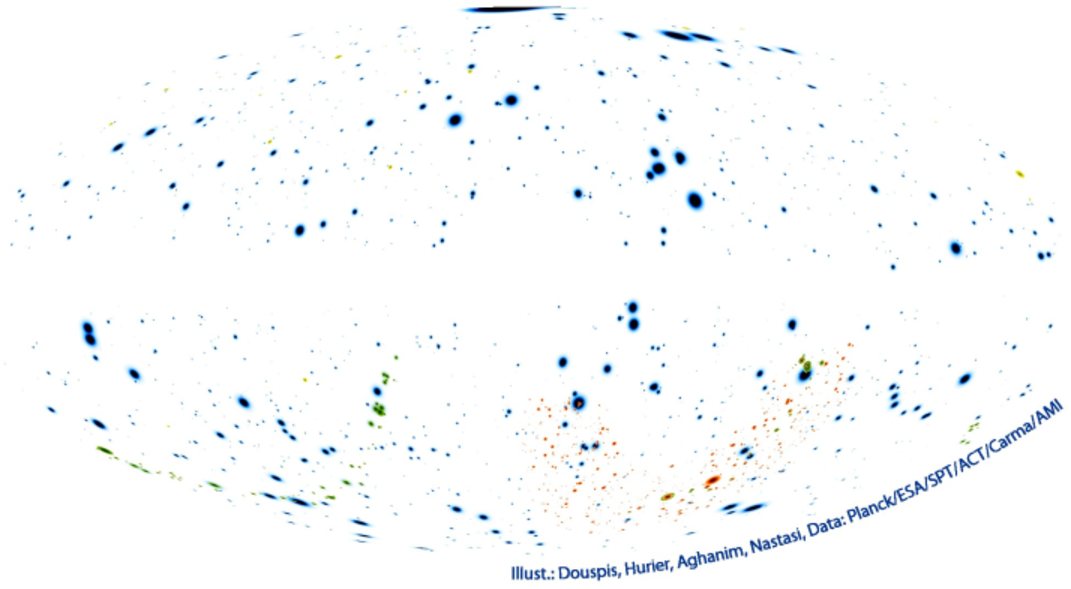
\includegraphics[width=0.9\columnwidth]{./Figures/Cat_all_colors_cr_DouspisEtAlCrop.pdf}
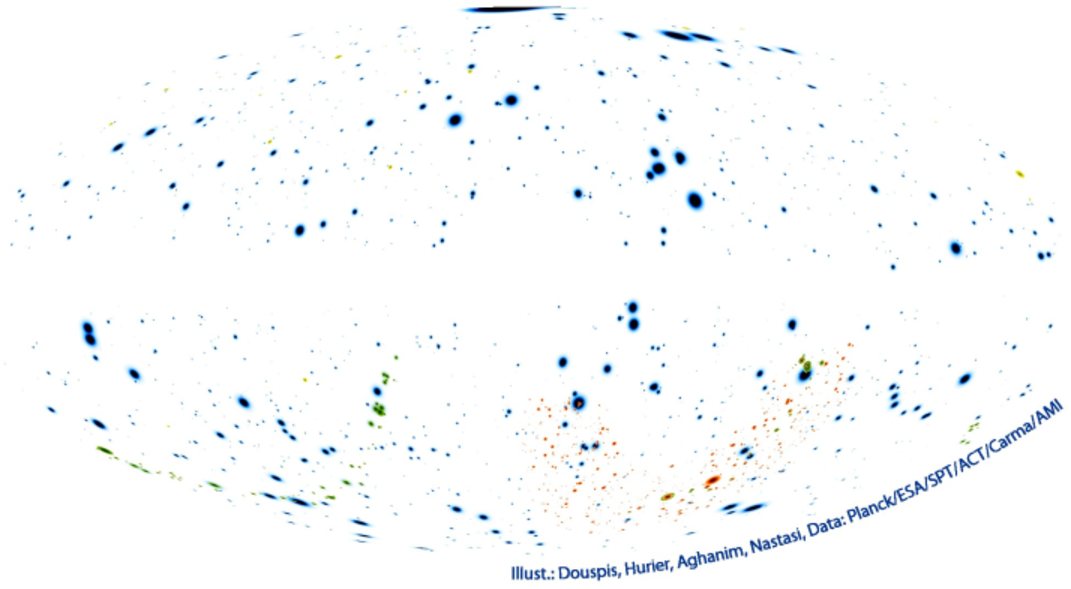
\includegraphics[width=0.45\columnwidth]{./Figures/Cat_all_colors_cr_DouspisEtAlCrop.pdf}
   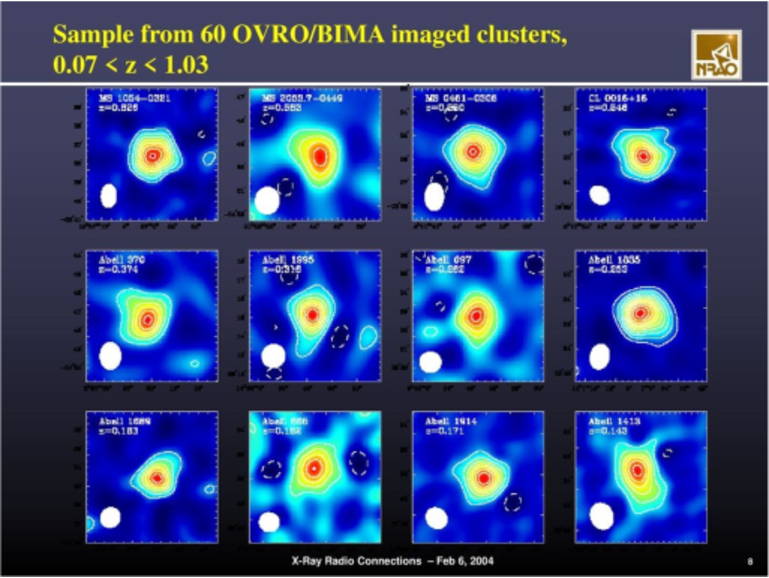
\includegraphics[width=0.45\columnwidth]{./Figures/slide_8crop.pdf}
  \end{center}
\caption{{\bf Left:} Visualization of an all-sky map of SZ clusters of galaxies, in galactic coordinates. Each dot is a cluster. Bigger dots are too extended for the present program. {\bf Right: } A sample of SZ maps obtained with OVRO/BIMA. \cite{Reese2002}}

\label{Fig:AllSky}
\end{figure}

%\begin{figure}
%  \begin{center}
%   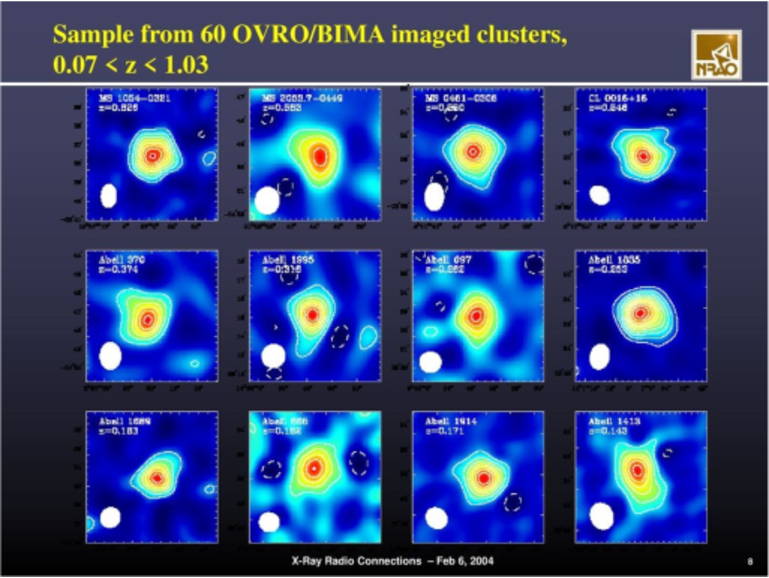
\includegraphics[width=0.4\columnwidth]{./Figures/slide_8crop.pdf}
%  \end{center}
%\caption{A sample of SZ maps obtained with OVRO/BIMA. Carlstrom et al.}
%\label{Fig:OVRO}
%\end{figure}

%\begin{figure}
%  \begin{center}
% 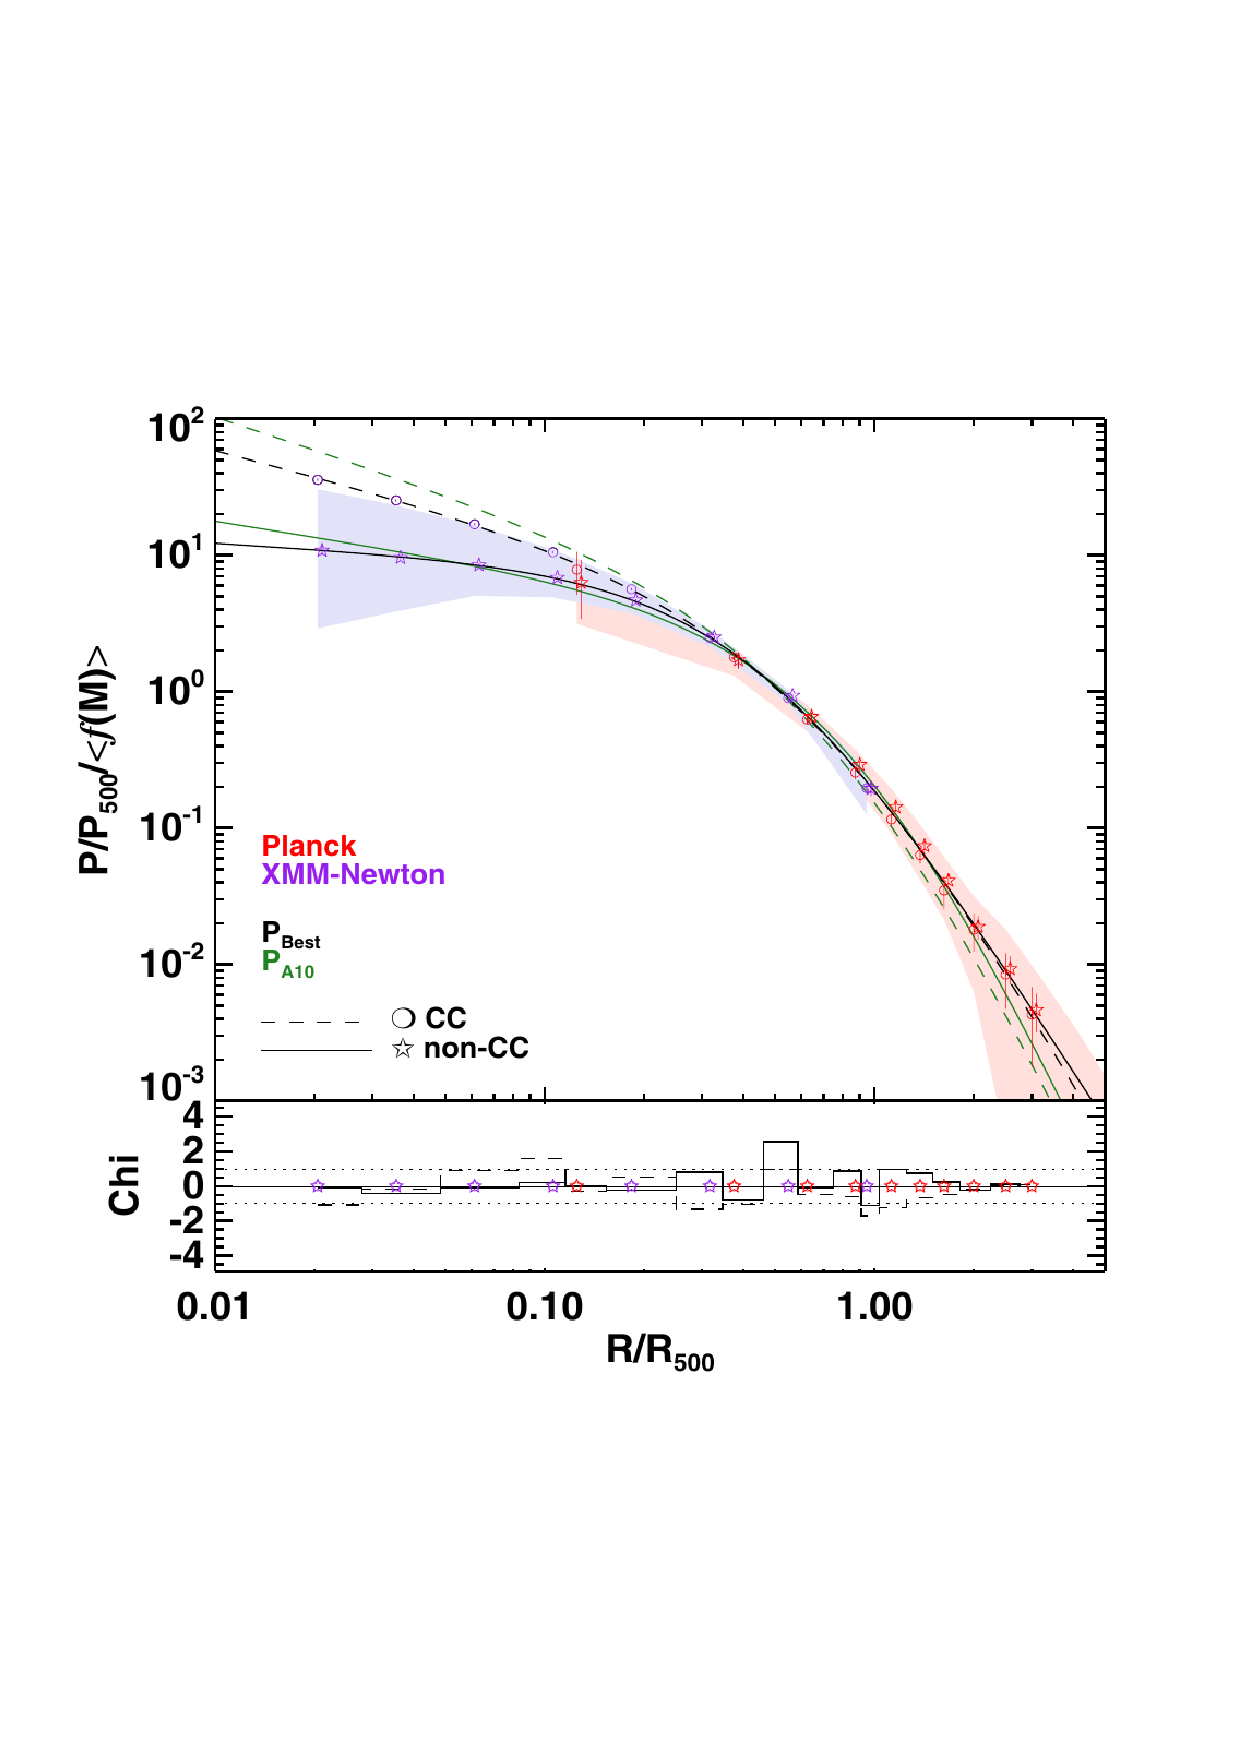
\includegraphics[width=0.9\columnwidth]{./Figures/PressureProfilePlanckXMM.pdf}
%  \end{center}
%\caption{Radial profile of the pressure in a standard {\sl Planck} cluster. The inner part is not well-known in SZ mode. The horizontal axis corresponds to 5~arcmin at 1. Cool core clusters differ in the center from non-cool-core clusters.}
%\label{Fig:PlanckXMM}
%\end{figure}

\begin{figure}
  \begin{center}
   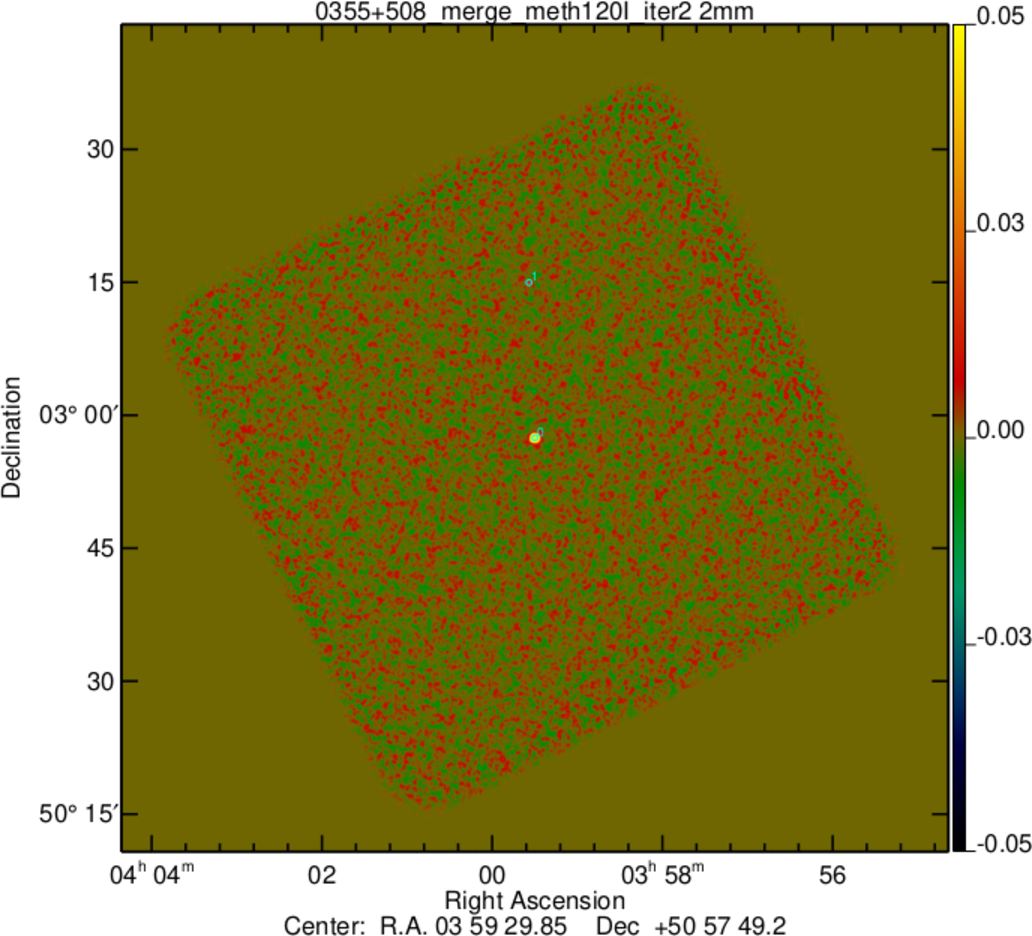
\includegraphics[width=0.3\columnwidth]{./Figures/0355+508_merge_meth120I_iter2_source_detect2mmCrop.pdf}
  \end{center}
\caption{One square-degree NIKA2 map obtained with a fast raster
  scan. It is centered on a typical 30~m pointing source.  The map
  covers more a one-degree square. It is made by co-adding 4 scans,
  each scan covering the total area either at +45 or -45 degrees from
  azimuth. This test case was obtained, just before enabling a
  polarization commissionning session, when the opacity was 0.57 at
  1~mm and 0.33 at 2~mm for an elevation of 34~degrees, conditions
  which are far from acceptable for normal scientific
  observations. The scan speed was 150~arcsecond/s to cover
  60~arcminutes per subscan (times 21~subscans to cover 60 arcmin in
  the cross direction). The scan duration was 10~minutes. The central
  source is well detected with a 2.8~Jy flux at 2~mm and a FWHM of
  less than 18~arcseconds, {\sl i.e.} no beam smearing effect from the
  scan speed and the same flux as with a normal intensity speed map. A
  serendipitous source of about $46\pm6\,\mathrm{mJy}$ is found within
  5~arcsecond of a Radio and WISE Source (WISEA J035933.92+511521.2
  has a 1.4~GHz flux of 24~mJy)}
\label{Fig:1sqdegMap}

\end{figure}

\begin{figure}
  \begin{center}
   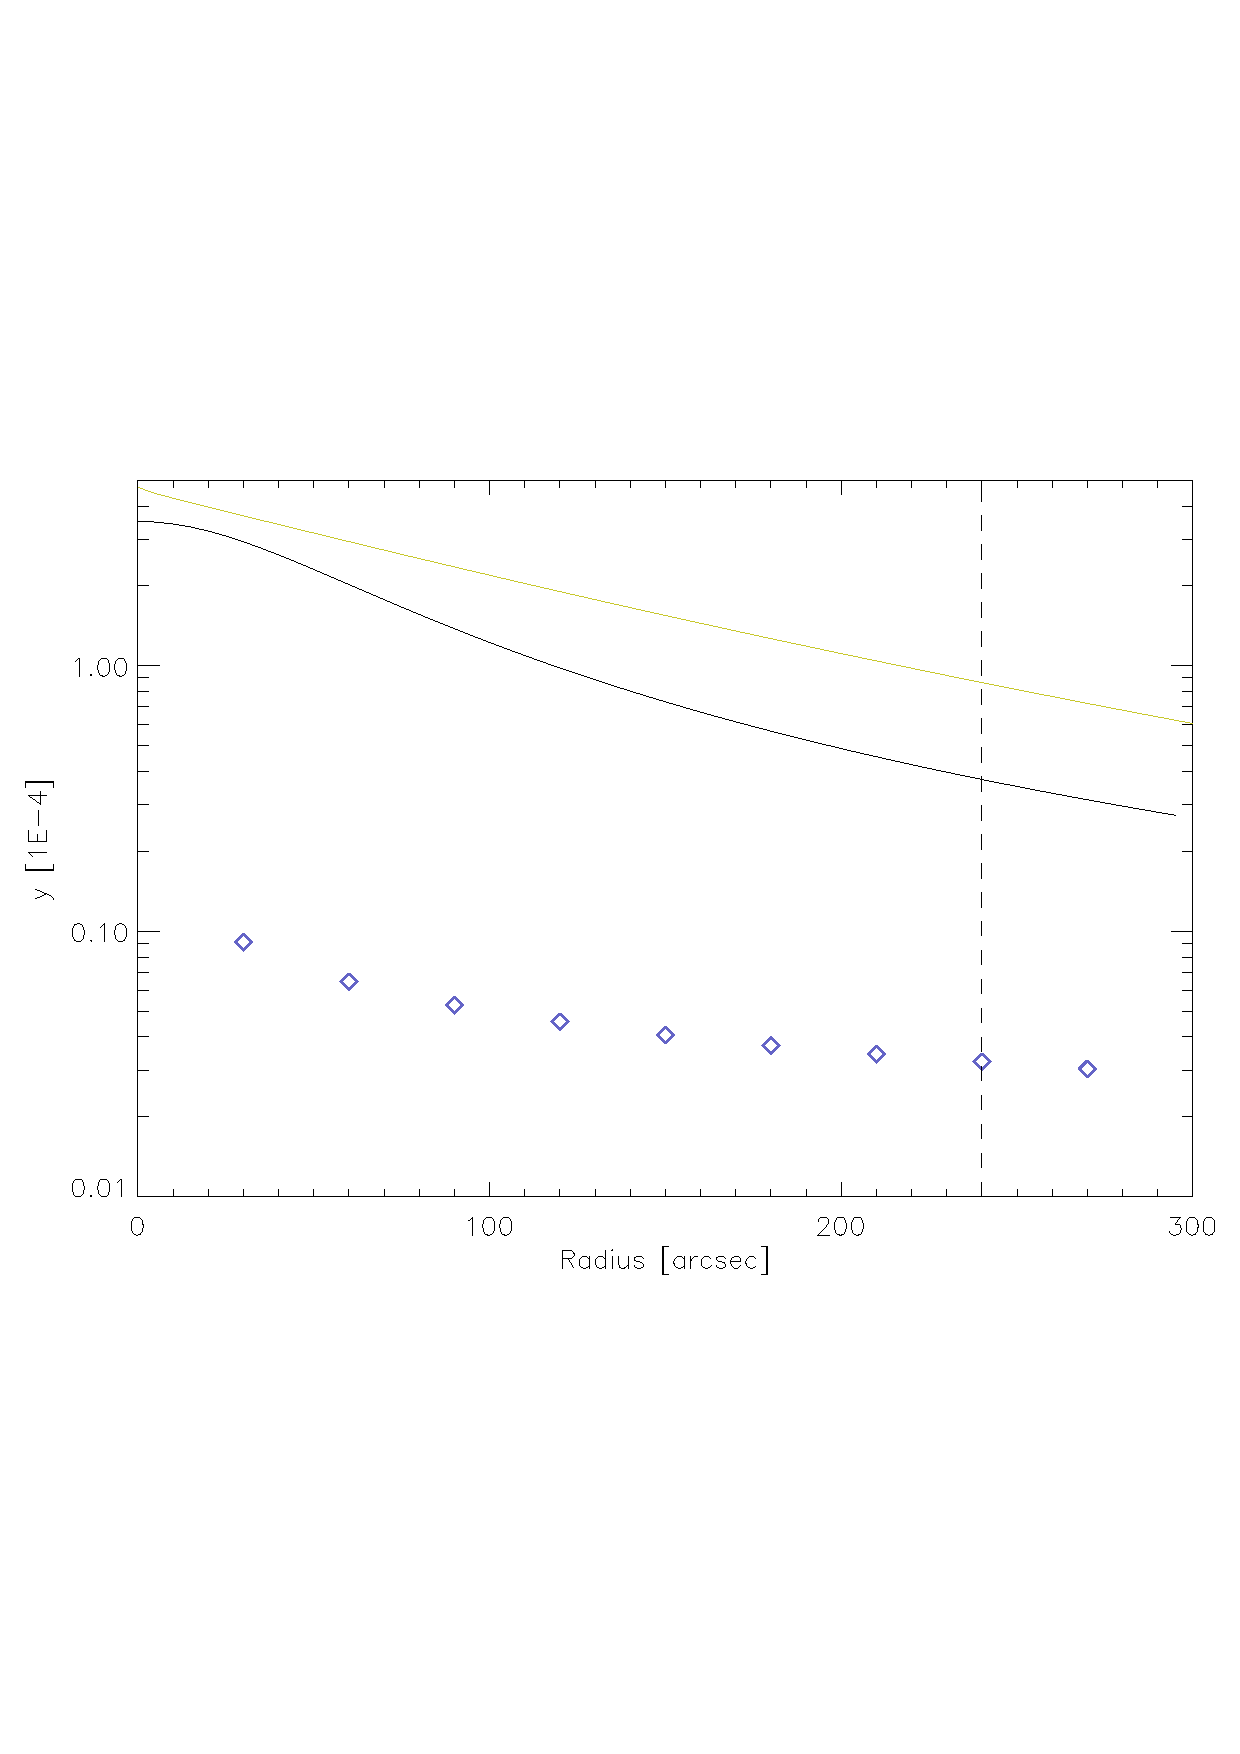
\includegraphics[width=0.45\columnwidth]{./Figures/Arsenal_SZprofile.pdf}
   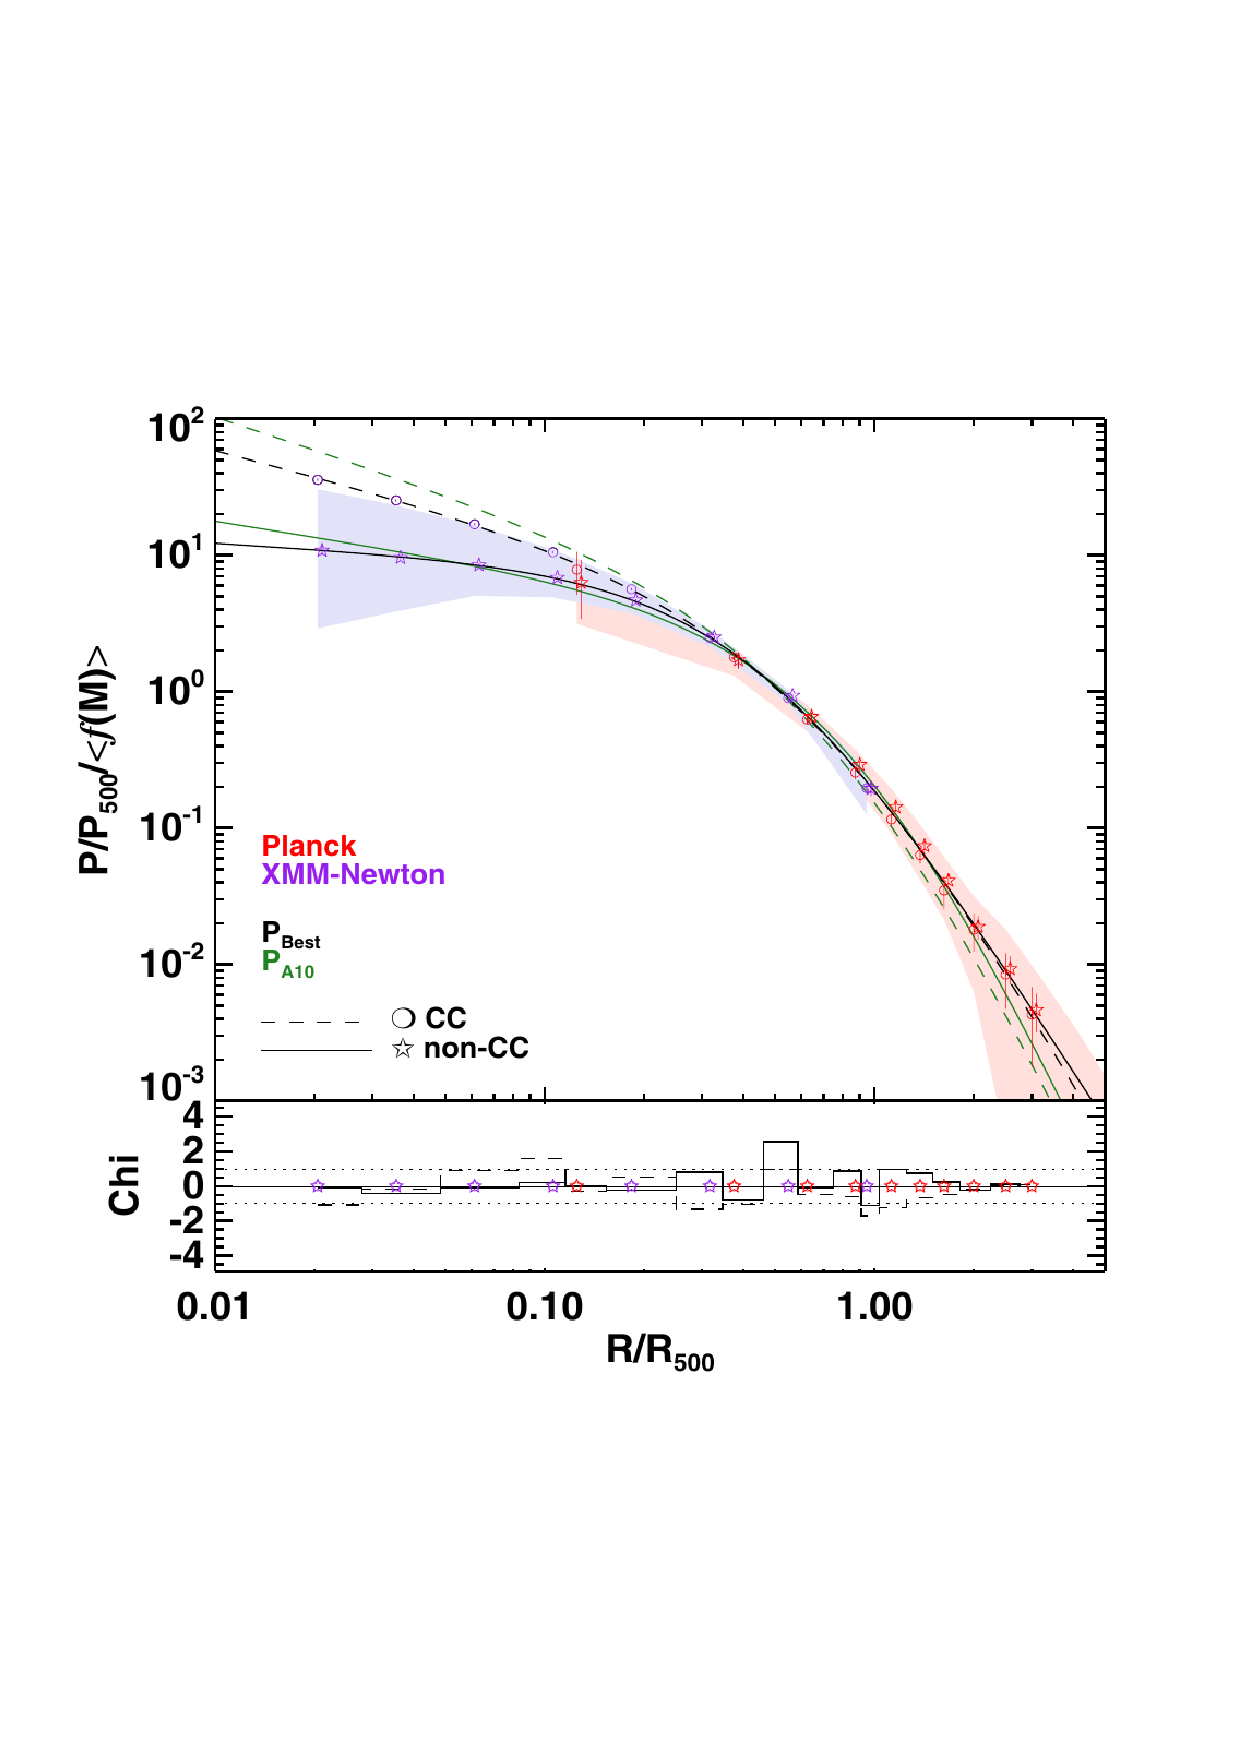
\includegraphics[width=0.45\columnwidth]{./Figures/PressureProfilePlanckXMM.pdf}
  \end{center}
  \caption{{\bf Left}~Radial profile of the SZ effect for a massive
    cluster (typically A2163) with a core radius of one arcminute. Two
    models are shown, the $\beta$ one being in black (derived from SZ
    data by \cite{Reese2002}) and the X-ray derived model from
    \cite{Arnaud2010} in yellow. Error bars for NIKA2 measurements in
    annuli are shown as diamonds (after 2 hours of observations). The
    recovery of large angular scales will be more difficult beyond the
    dashed line (8~arcmin diameter). {\sl Planck} clusters are on
    average less bright (2 to 10 times) than the example shown
    (A2163). The integration time will be modulated with each
    cluster. {\bf Right}~Radial profile of the pressure in a standard
    {\sl Planck} cluster. The inner part is not well-known in SZ
    mode. The horizontal axis corresponds to 5~arcmin at
    $R_{500}$. Cool core clusters differ in the center from
    non-cool-core clusters.}
  
\label{Fig:SZprofile}
\end{figure}
   
\begin{figure}
  \begin{center}
   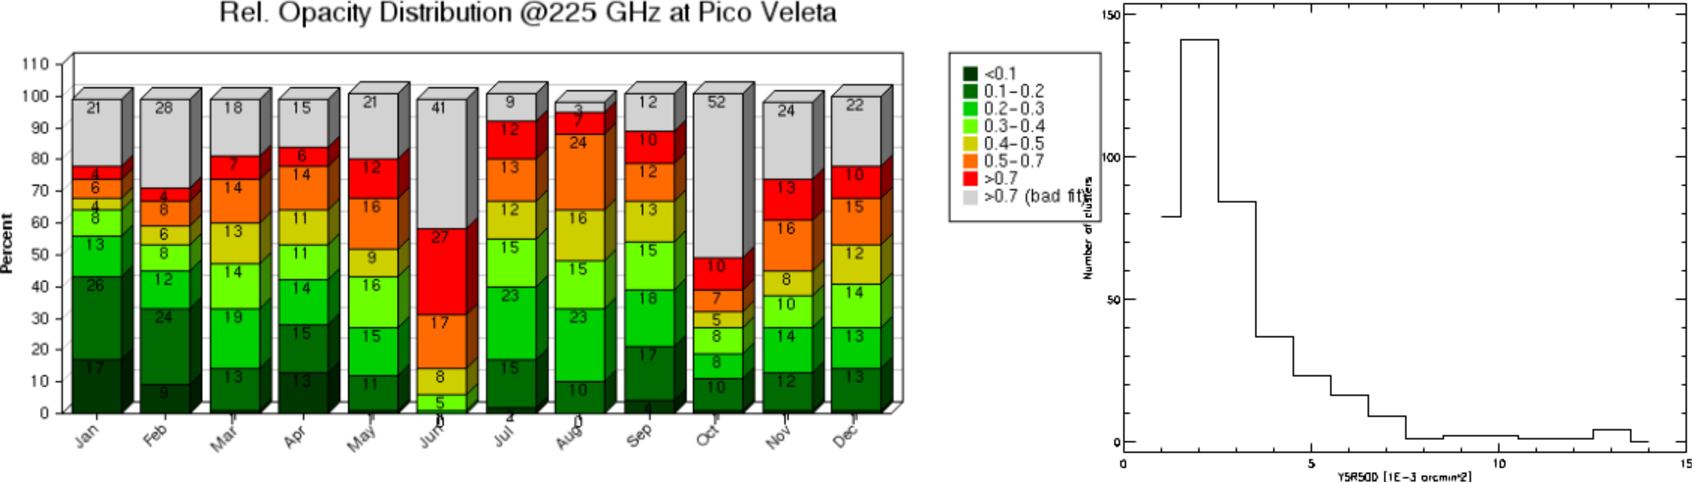
\includegraphics[width=0.95\columnwidth]{./Figures/RelTau2004AndSZclustersCrop.pdf}
  \end{center}
  \caption{{\bf Left}~Relative distribution of 225~GHz taumeter
    opacities during the 2003/2004 period. IRAM document.  {\bf
      Right}~Distribution in the integrated Compton parameters of the
    400~{\sl Planck} clusters detected above 3~$\sigma$ and with a
    declination above -15~degrees. No redshift selection was made
    here. }
\label{Fig:RelTau}
\end{figure}

%\begin{figure}
%  \begin{center}
%   %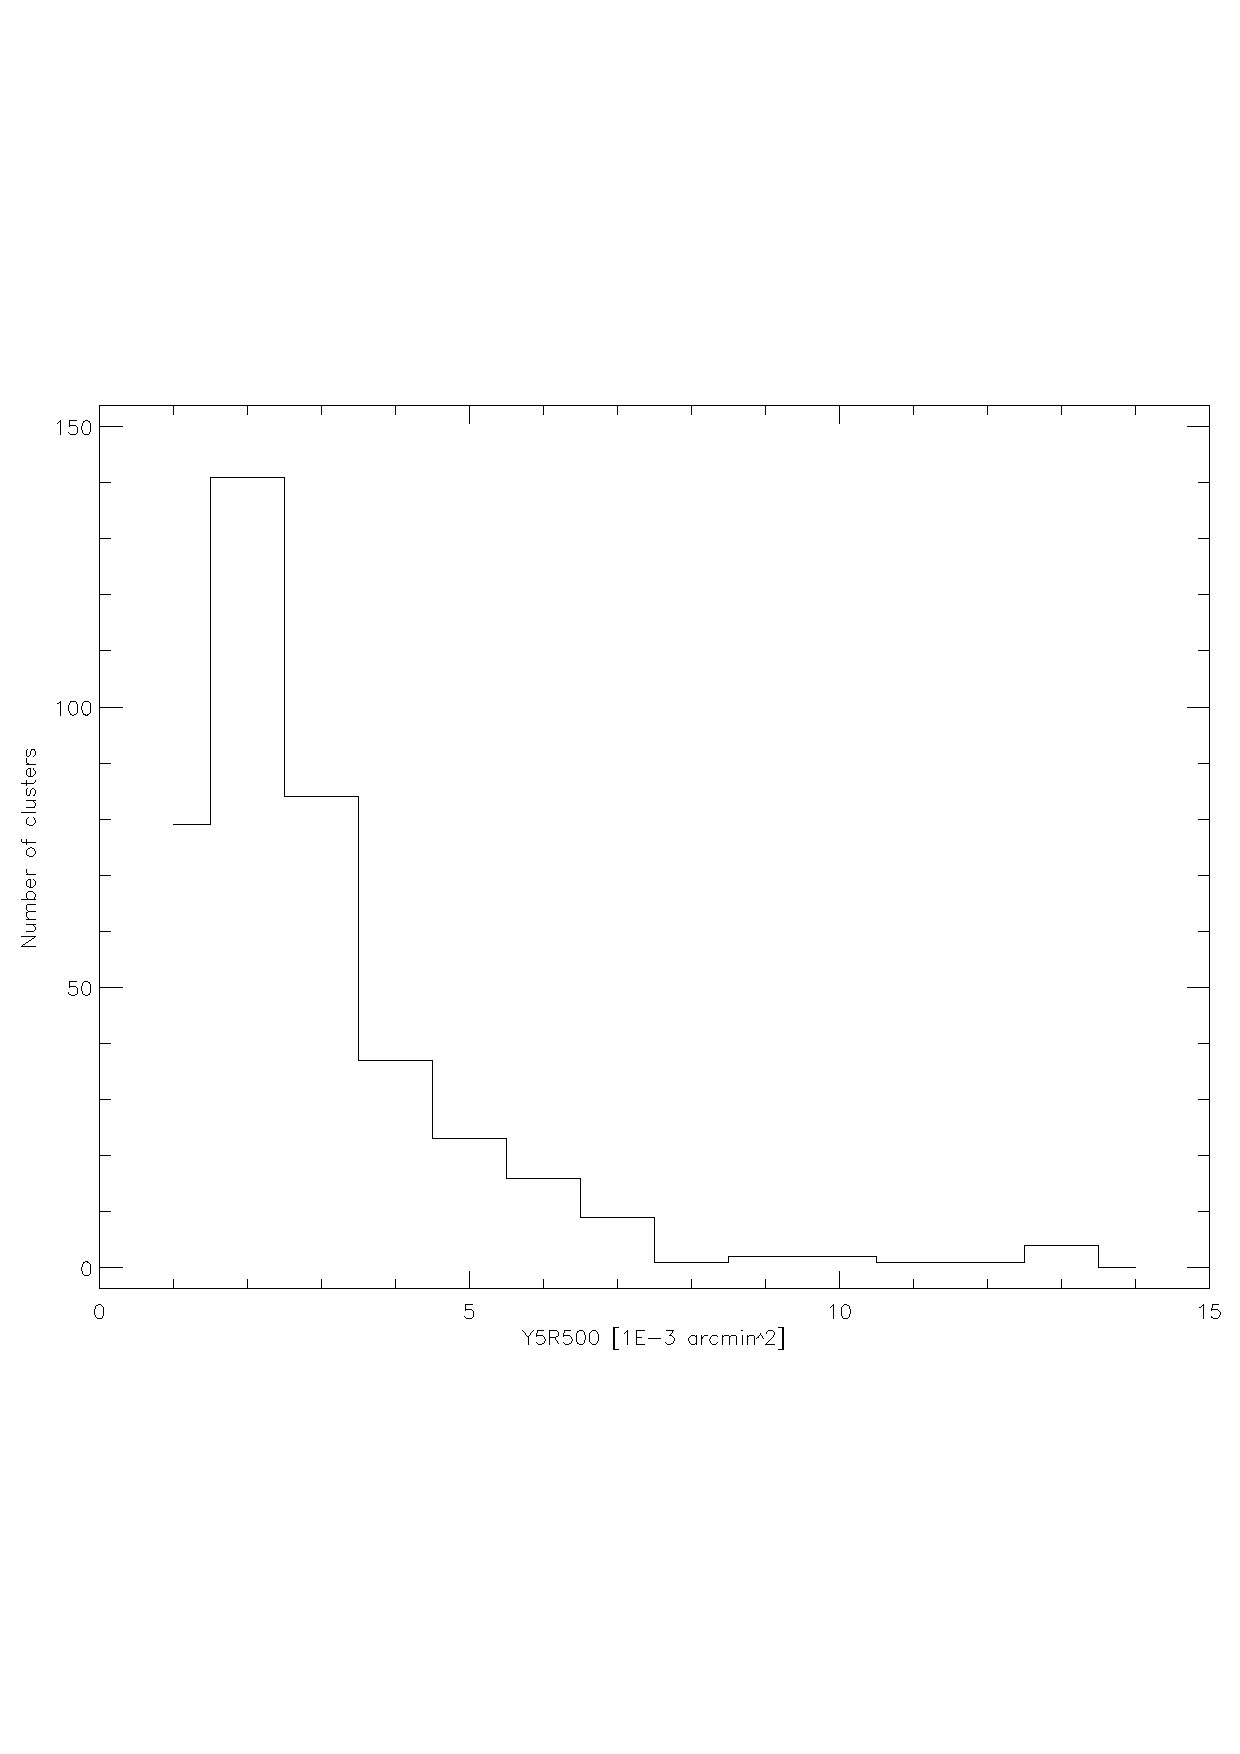
\includegraphics[width=0.9\columnwidth]{./Figures/Arsenal_SZclusters.pdf}
%  \end{center}
%\caption{ Distribution in the integrated Compton parameters of the %400~{\sl Planck} clusters detected above 3~$\sigma$ and with a %declination above -15~degrees. No redshift selection was made here.}
%\label{Fig:DistribClusters}
%\end{figure}



\end{document}
